Without loss of generality, let us focus on one particular source of uncertainty: the subthreshold leakage current and, more specifically, on the effective channel length. The reason for this choice is that the effective channel length has the strongest influence on leakage \cite{juan2011, juan2012}; in particular, it also affects the threshold voltage. Consequently, in what follows, $\u$ stands for this major parameter, the channel length.

\begin{figure}
  \centering
  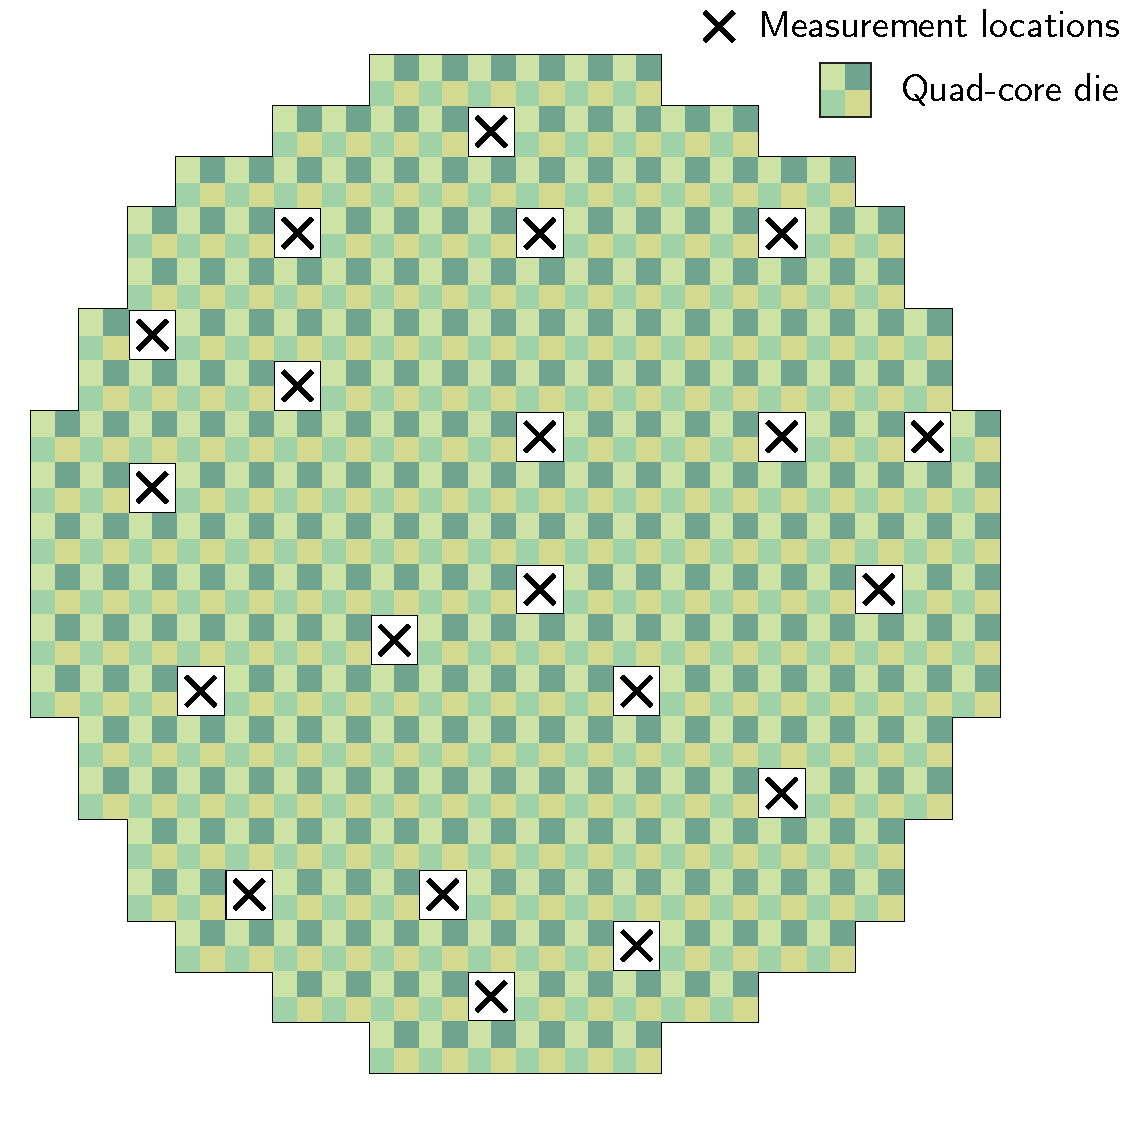
\includegraphics[width=0.7\linewidth]{include/assets/wafer-pick.pdf}
  \caption{A wafer with 316 quad-core dies.}
  \flabel{wafer-pick}
  \vspace{-1.5em}
\end{figure}

\begin{figure}[b]
  \centering
  \vspace{-1.5em}
  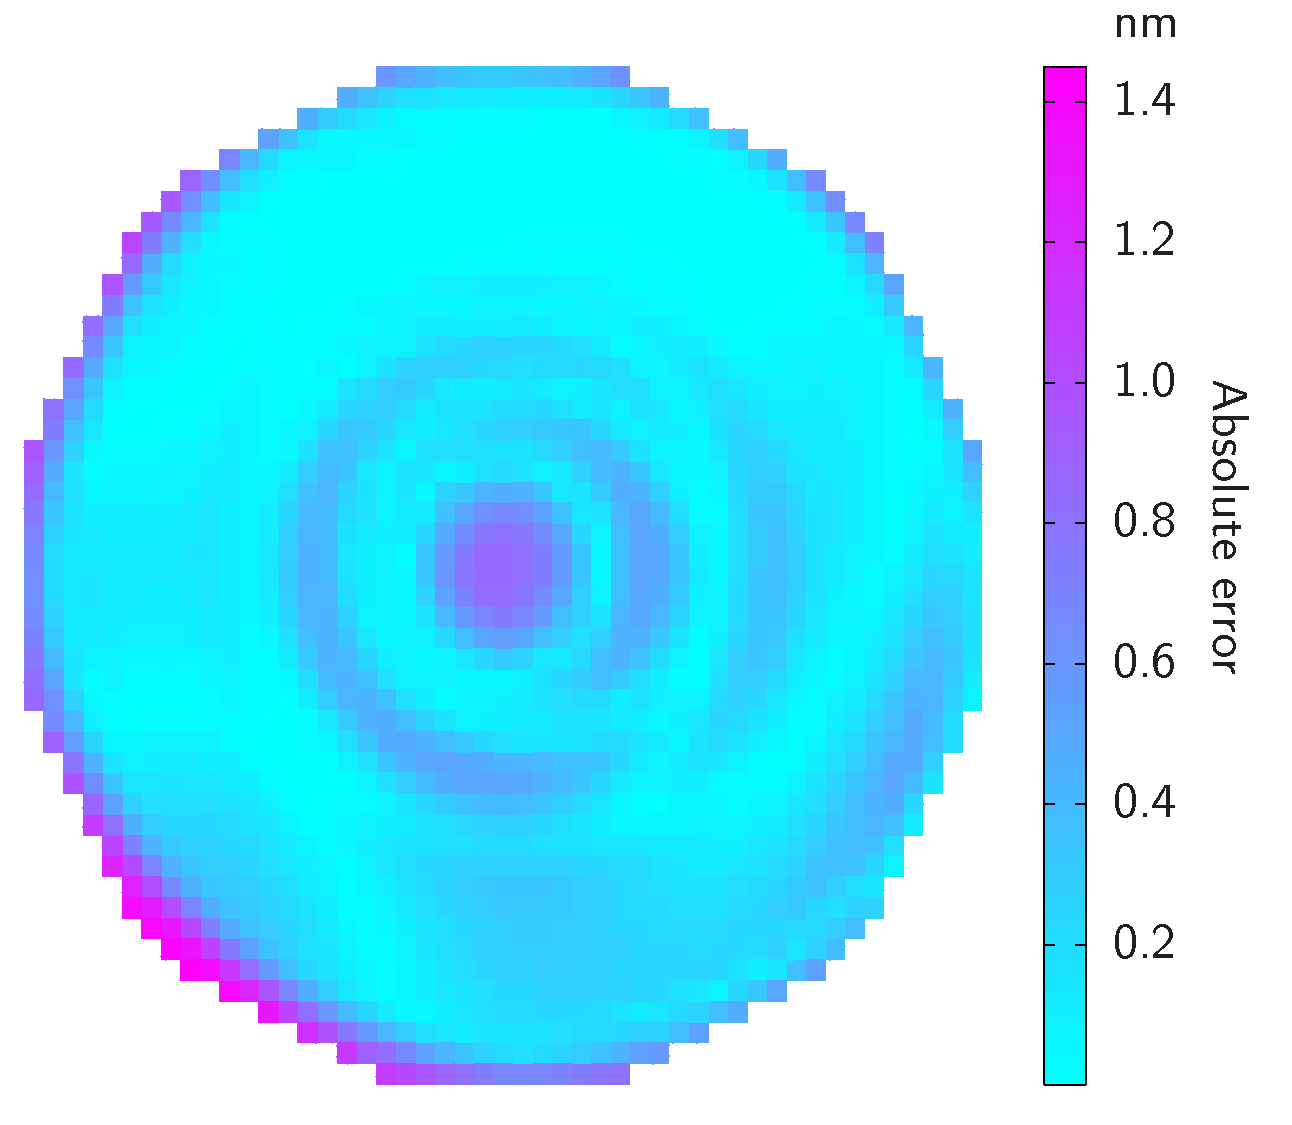
\includegraphics[width=0.6\linewidth]{include/figures/wafer-qoi-error.pdf}
  \caption{Distribution of the absolute error.}
  \flabel{wafer-qoi-error}
\end{figure}

Now, we shall describe the default configuration of our experimental setup, which, in the following subsections, will be adjusted according to the purpose of a particular experiment. We consider a 45-nanometer technological process. The wafer is assumed to be inscribed in a square with $20 \times 20$ even cells. The total number of dies $\nchips$ is 316, and the number of processing elements $\nprocs$ on each of the dies is four.
The number of spacial measurements $\ndata$ is 20. These locations (dies) are chosen as follows: the first one is place in the middle of the wafer, and the other are selected sequentially such that the total distance from the already picked dies and the new one to the rest of the dies is minimized. In this way, we pursue uniformity of the wafer coverage. An example is depicted in \fref{wafer-pick}.
The floorplans of the multiprocessor platforms are constructed in such a way that the processing elements form regular grids, as it is the case with, \eg, Alpha 21264 studied in \cite{juan2011}. The capacitance and conductance matrices in \eref{heat-de} are obtain using HotSpot v5.02 \cite{hotspot}. The dynamic power profiles involved in the experiments are based on simulations of randomly generated, via TGFF v3.5 \cite{dick1998}, task graphs.\footnote{The floorplans of the platforms, thermal configuration of HotSpot, task graphs of the applications, etc. are available online at \cite{sources}.} The number of power samples $\npsteps$ is $10^3$.
The corresponding temperature profiles that form the input data set $\Data$ are obtained as follows: (a) draw $\ndata$ samples of $\u$ for all processing elements on the wafer from a Gaussian distribution with mean $45~\text{nm}$ and the covariance function given by \eref{covariance-function}, wherein the standard deviation is $5\%$ \cite{juan2011, juan2012}; (b) for each such sample, simulate the thermal system in \eref{thermal-system} $\ndata$ times, once for each die, using the input dynamic power profile; (c) shrink the full temperature profiles to keep only $\nsteps$ (out of $\npsteps$) evenly spaced time moments; (d) perturb the data using a Gaussian white noise with the standard deviation equal to $1~\text{K}$ (Kelvin). By default, the number of temporal measurements $\nsteps$ is 20.

Let us turn to the statistical model in \sref{statistical-model}. In the covariance function given by \eref{covariance-function}, the weight parameter $\eta$ is 0.7 prioritizing the squared exponential kernel, and both length-scale parameters, $\ell_\SE$ and $\ell_\OU$, are set to half the radius of the wafer. The threshold parameter in the model order reduction procedure described in \sref{kl-expansion} is set to $0.99$ preserving $99\%$ of the variance of the data; the number of the resulting \rvs, \ie, the dimensionality of $\vz$ in \eref{kl-approximation}, $\nvars$, was found to be 27--28.
In the prior for the mean of $\u$ (see \eref{mu-u-prior}), we let $\mu_0$ be $45~\text{nm}$ and $\sigma_0$ be $1\%$ of $\mu_0$. The later represents our rather high certainty about the expected value of $\u$ as it is a part of the specification of the technological process.
In the prior for the variance of $\u$ (see \eref{sigma2-u-prior}), we let $\tau_\u$ be $5\%$ of the mean value, and $\nu_\u$ is set to ten. The later has an intuitive interpretation in the Bayesian context: $\nu_\u$ can be thought of as being the number of imaginary observations (prior to actual observations) that the decision about $\tau_\u$ is based on.
In the prior for the variance of noise (see \eref{sigma2-noise-prior}), we let $\tau_\noise$ be $1~\text{K}$, and $\nu_\noise$ be ten observations (the same meaning as for $\nu_\u$).
To summarize the reasoning behind the priors, the hyperparameters $\mu_0$, $\tau_\u$, and $\tau_\u$ represent the presumable values of $\mu_u$, $\sigma_\u$, and $\sigma_\noise$, respectively, and the hyperparameters $\sigma_0$, $\nu_\u$, and $\nu_\noise$ reflect the degree of our beliefs according to our prior knowledge. In the absence of such knowledge, non-informative priors can be chosen (see, \eg, \cite{gelman2004}).
In \eref{proposal}, the number of degrees of freedom $\nu$ is eight, and the tuning constant $\alpha$ is set to 0.5.
The optimization procedure (recall \sref{proposal-distribution}) is limited by $10^4$ objective function evaluations (the log-posterior in \eref{log-posterior}).
The number of samples that we draw from the posterior is $10^4$; the first half of these samples is discarded leaving $5 \cdot 10^3$ effective samples $\nsamples$.
Finally, in parallel computations, there are four workers employed.\footnote{All the experiments have been conducted on a GNU/Linux machine with Intel Core i7 2.66~GHz and 8~GB of RAM.}

\subsection{Analysis of the Experimental Setup}
\begin{figure}
  \centering
  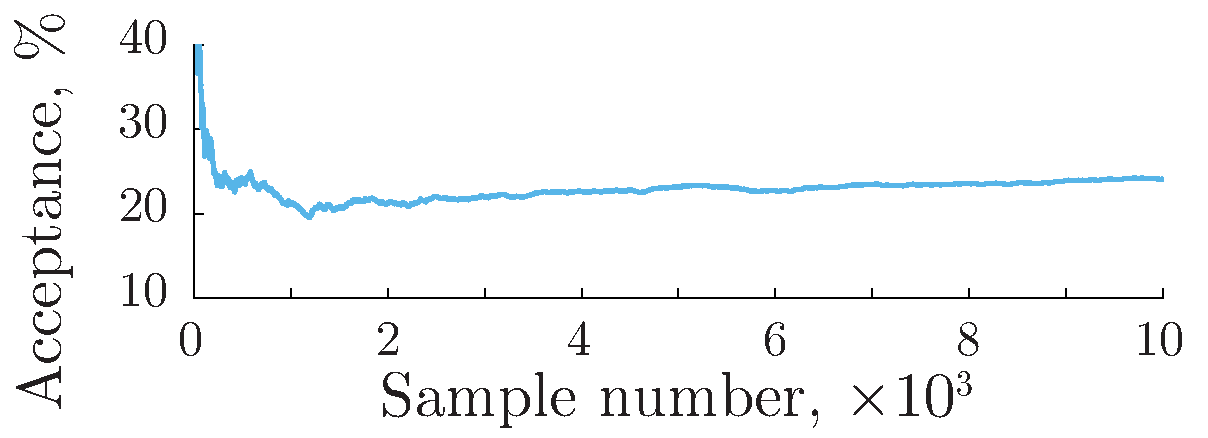
\includegraphics[width=0.7\linewidth]{include/figures/acceptance.pdf}
  \caption{Evolution of the acceptance rate.}
  \flabel{acceptance}
  \vspace{-0.5em}
\end{figure}

\begin{figure}
  \centering
  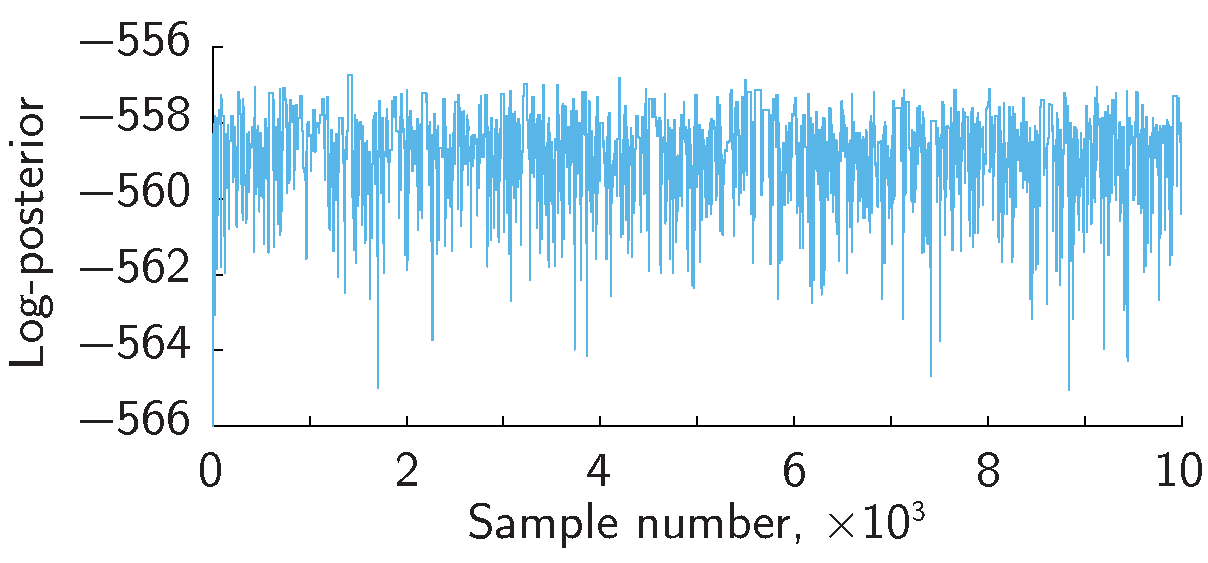
\includegraphics[width=0.7\linewidth]{include/figures/log-posterior.pdf}
  \caption{Evolution of the log-posterior.}
  \flabel{log-posterior}
  \vspace{-1.5em}
\end{figure}

\begin{figure}
  \centering
  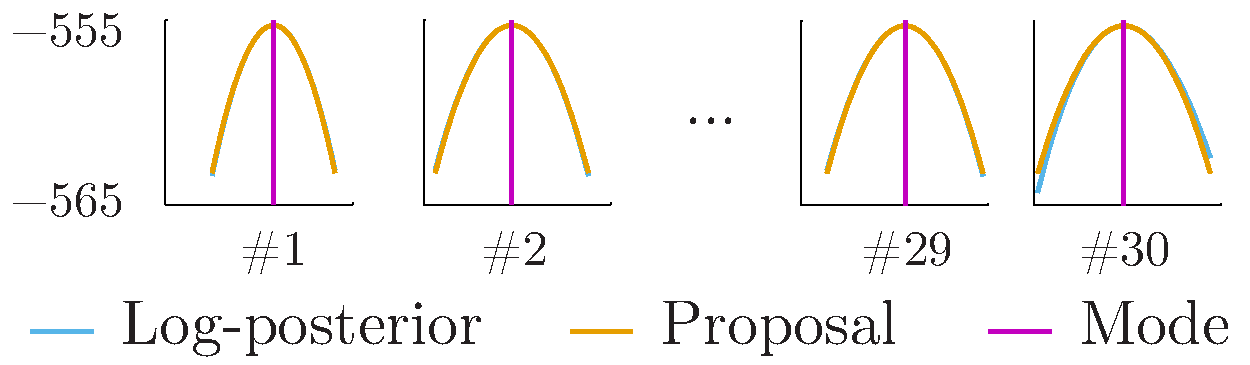
\includegraphics[width=0.8\linewidth]{include/figures/proposal.pdf}
  \caption{Inspection of the proposal.}
  \vspace{-1.5em}
  \flabel{proposal}
\end{figure}

In order to ensure that the experimental setup is adequate, let us first perform a detailed analysis of the results obtained for one particular example with the default configuration described earlier. The true and inferred distributions of the QoI are shown in \fref{wafer-qoi}. In this case, the normalized root-mean-square error (NRMSE) is below $2.8\%$, and the distribution of the absolute error across the wafer is visualized in \fref{wafer-qoi-error}. It can be seen that the framework produces a close match to the true value of the QoI.
\fref{acceptance} displays the acceptance rate of the Metropolis algorithm; this graph allows us to conclude that the algorithm, accepting $20$--$30\%$ of samples on average, agrees with the recommendations from the literature \cite{gelman2004}.
An inspection of the log-posterior depicted in \fref{log-posterior} (up to a constant summand) indicates that the constructed Markov chain vividly explores the probability space.
Another test, commonly used in statistics, to assess the quality of the proposal distribution is given in \fref{proposal}. Here, the log-posterior in \eref{log-posterior} and proposal in \eref{proposal} are plotted about the posterior mode $\hat{\vparam}$ (see \sref{proposal-distribution}). Since, in this example, the dimension of $\vparam$ is 30, the number of such plots is also 30. The curves are nearly indistinguishable implying a high quality of the proposal. To sum up, the above observations suggest that the optimization and sampling procedures are fine-tuned.

\subsection{Number of Processing Elements}
In this subsection, we consider five platforms with the number of processing elements $\nprocs$ equal to 2, 4, 8, 16, and 32 cores, respectively. The results are summarized in \tref{processing-elements}. In this and the following tables, we report the optimization and sampling times separately; also, the sampling time is given for two cases: sequential and parallel computing (with four workers), which is followed by the total time and error. The sequential sampling time is the most representative indicator of the computational complexity changes as the number of samples is always fixed, and there is no parallelization; thus, we shall refer to it in most of the discussions below.
\begin{table}[h]
  \centering
  \caption{Results for the number of processors $\nprocs$.}
  \begin{tabular*}{1\linewidth}{=l@{\hskip 4em}-r-r-r-r-r}
    \toprule
    Processing elements    & 2 & 4 & 8 & 16 & 32 \\
    \midrule
    \midrule
    Optimization time, m   & 2.67 & 3.34 &  5.20 &  7.37 & 13.85 \\
    \midrule
    \rowstyle{\bfseries}
    Sequential sampling, m & 3.71 & 4.60 &  6.03 &  8.92 & 14.77 \\
    Total time, m          & 6.38 & 7.94 & 11.23 & 16.29 & 28.62 \\
    \midrule
    Parallel sampling, m   & 0.98 & 1.18 &  1.58 &  2.51 & 5.30 \\
    Total time, m          & 3.65 & 4.52 &  6.78 &  9.88 & 19.15 \\
    \midrule
    NRMSE, \%              & 4.71 & 3.42 &  3.68 &  2.73 &  1.94 \\
    \bottomrule
  \end{tabular*}
  \tlabel{processing-elements}
  \vspace{-1em}
\end{table}


It can be seen that the computational time increases (the difference between the sequential and parallel setups is discussed later on). This behavior is expected as each processing element introduces additional complexity in the thermal system given by \eref{thermal-system}; more precisely, it leads to a larger number of thermal nodes $\nnodes$. Nevertheless, even for large examples, the timing is readily acceptable, taking into account the complexity of the inference procedure behind and the yielded accuracy.
An interesting observation can be made from the error metric (NRMSE): the error tends to decrease as the number of processing elements grows. The explanation is that, with each core, the data set $\Data$ delivers more information to the inference to work with since the temperature profiles in $\Data$ are being collected for all the cores simultaneously.

\subsection{Number of Spatial Measurements}
\begin{figure}
  \centering
  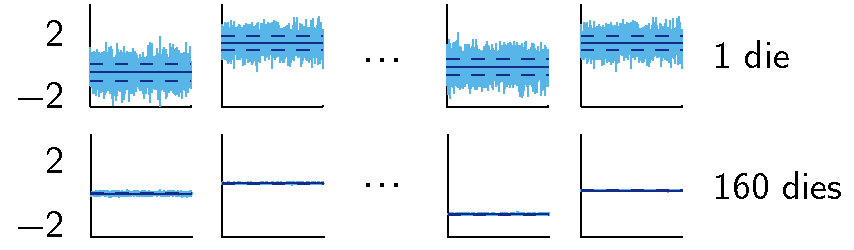
\includegraphics[width=0.8\linewidth]{include/assets/chains.pdf}
  \caption{Evolution of the Markov chains.}
  \flabel{chains}
  \vspace{-1.5em}
\end{figure}

In this subsection, we change the number of dies $\ndata$ for which the measurement data are available in the input data set $\Data$ (correspondingly, $\nchips - \ndata$ dies on the wafer are left unobserved). The considered scenarios are 1, 10, 20, 40, 80, and 160 dies. The results are reported in \tref{spatial-measurements}.
\begin{table}[h]
  \centering
  \caption{Results for the number of measured dies.}
  \begin{tabular*}{1\linewidth}{=l@{\hskip 4pt}-r-r-r-r-r-r}
    \toprule
    Measured dies   & 1 & 10 & 20 & 40 & 80 & 160 \\
    \midrule
    \midrule
    Optimization time, m   &  0.41 & 2.49 & 3.34 &  4.59 &  7.33 & 10.29 \\
    \midrule
    \rowstyle{\bfseries}
    Sequential sampling, m &  2.40 & 3.99 & 4.60 &  5.79 &  8.49 & 12.96 \\
    Total time, m          &  2.81 & 6.47 & 7.94 & 10.38 & 15.81 & 23.25 \\
    \midrule
    Parallel sampling, m   &  0.61 & 1.02 & 1.18 &  1.51 &  2.16 &  3.62 \\
    Total time, m          &  1.02 & 3.50 & 4.52 &  6.10 &  9.49 & 13.91 \\
    \midrule
    NRMSE, \%              & 30.49 & 4.40 & 3.42 &  1.09 &  0.85 &  0.67 \\
    \bottomrule
  \end{tabular*}
  \tlabel{spatial-measurements}
  \vspace{-1.5em}
\end{table}


We see that the more data the proposed framework needs to process, the longer the execution time, which is reasonable. The trend, however, is not as steep as the one in \tref{processing-elements} since the thermal system stays unchanged.
The NRMSE firmly decreases and drops below $4\%$ with around 20 die measurements, which is only $6.3\%$ of the total number of dies on the wafer.

Now, this example is a great opportunity to draw attention to an important advantage of being Bayesian, which has already been lit on one side in \sref{motivation}: the inference can tell us how uncertain its predictions are. In \tref{spatial-measurements}, we have two extreme cases: one die and 160 dies. It is reasonable to anticipate that the predictions are less accurate in the former case than those in the latter, and this is exactly what the NRMSE has revealed in \tref{spatial-measurements}. In reality, unfortunately, the true values and, consequently, errors are unknown. However, based on the sample draws from the posterior distribution---which also incorporates our prior knowledge coming, \eg, from experts in the present area---we can deduce how reliable the collected data in $\Data$ are. In particular, we can inspect the paths of the constructed chains. Several such paths for the current example are depicted in \fref{chains} where the top and bottom rows correspond to one and 160 die measurements, respectively. The message to be taken here is that the variance of the one-die case is much larger than the one of the 160-die scenario.

\subsection{Number of Temporal Measurements}
In this subsection, we sweep the number of moments of time $\nsteps$ for which the measurement data are available in the input data set $\Data$ (correspondingly, $\npsteps - \nsteps$ steps are discarded after $\model$ is evaluated for the input power profile $\profilePdyn$). The considered scenarios are 1, 10, 20, 40, 80, and 160 moments of time. The results are aggregated in \tref{temporal-measurements}.
\begin{table}[h]
  \vspace{-1.5em}
  \centering
  \caption{Results for the number of temporal measurements.}
  \begin{tabular*}{1\linewidth}{=l-r-r-r-r-r-r}
    \toprule
    Temporal measurements  & 1 & 10 & 20 & 40 & 80 & 160 \\
    \midrule
    \midrule
    Optimization time, m   & 1.12 & 3.02 & 3.34 & 3.62 & 3.64 & 4.20 \\
    \midrule
    \rowstyle{\bfseries}
    Sequential sampling, m & 2.40 & 4.38 & 4.60 & 4.67 & 4.80 & 4.97 \\
    Total time, m          & 3.52 & 7.40 & 7.94 & 8.29 & 8.44 & 9.16 \\
    \midrule
    Parallel sampling, m   & 0.62 & 1.13 & 1.18 & 1.22 & 1.25 & 1.30 \\
    Total time, m          & 1.74 & 4.16 & 4.52 & 4.84 & 4.89 & 5.50 \\
    \midrule
    NRMSE, \%              & 7.48 & 2.72 & 3.42 & 1.83 & 2.34 & 1.32 \\
    \bottomrule
  \end{tabular*}
  \tlabel{temporal-measurements}
  \vspace{-0.5em}
\end{table}


As we see, the growth of the computational time is relatively low. One might have expected this time to be the same as the one for the spatial measurements since, formally, their influence on the dimensionality of $\Data$ is identical (recall $\ndps \propto \ndata \nsteps$). However, the meaning of the two numbers, $\ndata$ and $\nsteps$, is completely different, and, therefore, the way they manifest themselves in the algorithm is also different. Thus, the corresponding amounts of extra data are being treated differently leading to the divergent timing shown in \tref{spatial-measurements} and \tref{temporal-measurements}.
The NRMSE in \tref{temporal-measurements} is decreasing on average; however, the observed trend is less steady than the ones discovered before. The finding can be explained as follows. The distribution of the time moments in $\Data$ changes since these moments are kept evenly spaced across the corresponding time spans of the input power profiles. Some time moments can be more informative than the other. Consequently, more representative or less representative samples can end up in $\Data$ helping or misleading the inference procedure.
Based on \tref{spatial-measurements} and \tref{temporal-measurements}, we also conclude that a larger number of spatial measurements is more advantageous for the inference than a larger number of temporal measurements.

\subsection{Measurement Noise}
In this subsection, we vary the level of the noise in the input data set $\Data$ within the set $\{ 0, 0.5, 1, 2 \}$ (in Kelvins). Note that the corresponding prior distribution in \eref{sigma2-noise-prior} is kept unchanged. The results are given in \tref{noise-deviation}.
\begin{table}[h]
  \centering
  \caption{Results for the level of the measurement noise.}
  \begin{tabular*}{1\linewidth}{=l@{\hskip 5.5em}-r@{\hskip 2em}-r@{\hskip 2em}-r@{\hskip 2em}-r}
    \toprule
    Deviation of the noise & 0, K & 0.5, K & 1, K & 2, K \\
    \midrule
    \midrule
    Optimization time, m     & 5.08 & 3.73 & 3.34 & 3.19 \\
    \midrule
    \rowstyle{\bfseries}
    Sequential sampling, m   & 4.76 & 4.70 & 4.60 & 4.71 \\
    Total time, m            & 9.84 & 8.43 & 7.94 & 7.90 \\
    \midrule
    Parallel sampling, m     & 1.19 & 1.17 & 1.18 & 1.18 \\
    Total time, m            & 6.27 & 4.91 & 4.52 & 4.37 \\
    \midrule
    NRMSE, \%                & 0.02 & 2.71 & 3.42 & 4.05 \\
    \bottomrule
  \end{tabular*}
  \tlabel{noise-deviation}
  \vspace{-1em}
\end{table}


The computational time is approximately constant; the slight decrease with the decrease of the noise level can be ascribed to wider possibilities of perfection for the optimization procedure.
A more important observation, revealed by the experiment, is that, in spite of the fact that the inference operates on indirect and drastically incomplete data, a thoroughly calibrated equipment can considerably improve the quality of prediction. However, even with a high noise level of two degrees---meaning that all measurements fall on the band of $8~\text{K}$ wide around the true values with probability more than $0.95$---the NRMSE is still only $4\%$.

\subsection{Sequential vs. Parallel Sampling}
In this subsection, we summarize the results of the two sampling strategies: sequential and parallel (see \sref{sampling-strategy}). Since the limit on the number of objective function evaluations of the optimization procedure and the number of sample draws (including the burn-in prior) is the same, \ie, equal to $10^4$, the two would take the same time to finish if the optimization reached the limit. In our experiments, however, this limit was never observed to be reached. Therefore, using the default setup without parallelization, the optimization always takes less time than sampling. The situation changes when parallel computing (with four workers, in our case) is plugged in: the sampling part decreases by approximately 2–3 times, which indicates good parallelization properties of the chosen sampling strategy.
